\section{Morphological Thinning}
\begin{frame}
  \frametitle{Morphological Thinning}
  \textbf{Morphological Thinning}~\cite{morph} is a morphological operation that removes contour pixels from a region of a binary image. It relies on the \textbf{Hit-or-Miss transform} operation.
  \begin{block}
    {Hit-or-Miss transform}
    General binary morphological operation used to look for the presence of specific patterns of \emph{foreground} and \emph{background pixels} (1s or 0s respectively).
  \end{block}
  \begin{columns}
    \begin{column}{0.7\textwidth}
      \begin{itemize}
        \item Hit-or-Miss transform uses a \emph{structuring element} or \emph{kernel} to look for those patterns. \item Tipycally it is used a $3\times3$ kernel. It can contain both 1s and 0s and a special "I don't care" value.
        \item Iteration over all pixels, comparing the kernel with the underlying sub-image.
        \item \lstinline{M[i][j]}$= \begin{cases} 1 & \mbox{if } kernel =$ \lstinline{M[i-1:i+1][j-1:j+1]}$ \\ 0 & otherwise\end{cases}$
      \end{itemize}
    \end{column}
    \begin{column}{0.3\textwidth}
      \begin{figure}
        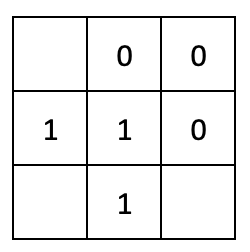
\includegraphics[width=0.8\textwidth]{hit-and-miss-kernel.png}
        \caption{Example of kernel. Cells in blank are "I don't care" valued.}
      \end{figure}
    \end{column}
  \end{columns}
\end{frame}

\begin{frame}[c]
  \frametitle{Morphological Thinning}
  \begin{block}
    {Thinning operation}
    Given a binary image $I$ and a kernel $K$:
    \begin{equation}
      thin(I, K) = I - hit\mbox{-}or\mbox{-}miss(I, K)
    \end{equation}
    where the subtraction is the logical subtraction $X-Y = X \cap \neg Y$
  \end{block}
  \begin{itemize}
    \item A pixel $(i, j)$ is deleted (i.e. set to 0) if kernel and sub-image \textbf{do not} exacly match, otherwise is left unchanged.
    \item To obtain a skeleton of the image, $thin(I, K)$ should be repeated until no change occurs.
    \item The choice of the kernel determines which pixels are deleted from the region.
  \end{itemize}
\end{frame}

\begin{frame}
  \frametitle{Skeletonization Kernels}
  \begin{itemize}
    \item Recalling Slide~\ref{sli:skeleton} a skeleton should preserve topological characteristics of the region such as connectivity, holes, cavities etc.
    \item $thin(I, K)$ deletes pixels based on the kernel K.
    \item The two kernels below (and all their 90° rotations) allow to delete only pixels whose deletion preserves the above mentioned characteristics.
    \item In each iteration $thin(I, K)$ is executed for each of the 8 resulting kernels.
  \end{itemize}
  \begin{figure}
    \centering
    \begin{subfigure}[b]{0.45\textwidth}
      \centering
      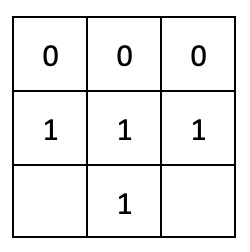
\includegraphics[width=0.6\textwidth]{border-kernel.png}
      \caption{Detects deletable border pixels.}
    \end{subfigure}
    \hfill
    \begin{subfigure}[b]{0.45\textwidth}
      \centering
      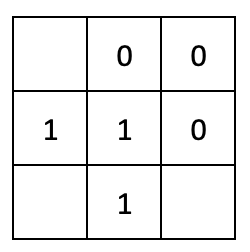
\includegraphics[width=0.6\textwidth]{corner-kernel.png}
      \caption{Detects deletable corner pixels.}
    \end{subfigure}
    \caption{Morphological thinning kernels (and all their 90° rotations)}
  \end{figure}
\end{frame}

\begin{frame}
  \frametitle{Spurs Problem}
  \begin{block}{Spurs}
    Skeletons obtained by $thin(I, K)$ with kernels presented in the previous slide can present \textbf{short spurs} produced by irregularities in the boundary of the region as shown below.
  \end{block}
  \begin{columns}
    \begin{column}{0.4\textwidth}
      \begin{figure}
        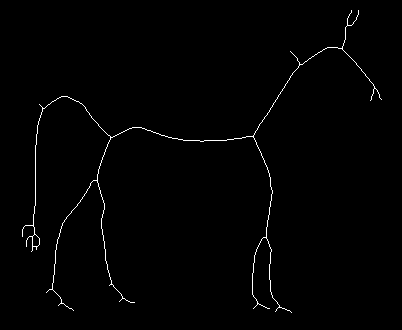
\includegraphics[width=\textwidth]{spur-example.png}
        \caption{Morphological thinning skeleton with spurs.}
      \end{figure}
    \end{column}
    \begin{column}{0.6\textwidth}
      \begin{itemize}
        \item Spurs can be removed by a process called \textbf{pruning}.
        \item Pruning is performed by applying $thin(I, K)$ with ad-hoc kernels for a \textbf{fixed amount} of iterations.
        \item Pruning until convergence would actually remove all pixels exept those which form closed loops.
      \end{itemize}
    \end{column}
  \end{columns}
\end{frame}

\begin{frame}
  \frametitle{Kernels for Spur Removal}
  By using the kernels (and all their 90° rotations) shown below it is possible to remove spurs from skeleton.
  \begin{columns}
    \begin{column}{0.5\textwidth}
      \begin{figure}
        \centering
        \begin{subfigure}[b]{0.5\textwidth}
          \centering
          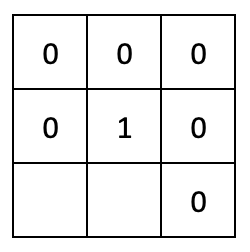
\includegraphics[width=\textwidth]{spur-1-kernel.png}
        \end{subfigure}
        \hfill
        \begin{subfigure}[b]{0.5\textwidth}
          \centering
          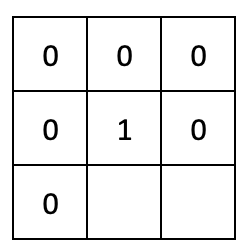
\includegraphics[width=\textwidth]{spur-2-kernel.png}
        \end{subfigure}
        \caption{Spur removal kernels.}
      \end{figure}
    \end{column}
    \begin{column}{0.5\textwidth}
      After removing spurs for 10 iterations we get the following skeleton.
      \begin{figure}
        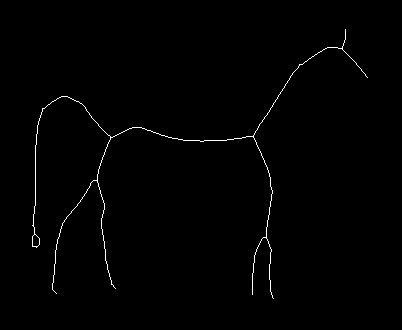
\includegraphics[width=\textwidth]{spur-removed.png}
        \caption{Skeleton after spur removal.}
      \end{figure}
    \end{column}
  \end{columns}
\end{frame}

\begin{frame}
  \frametitle{Morphological Thinning Pseudocode}
  \section{Morphological Thinning}
\begin{frame}
  \frametitle{Morphological Thinning}
  \textbf{Morphological Thinning}~\cite{morph} is a morphological operation that removes contour pixels from a region of a binary image. It relies on the \textbf{Hit-or-Miss transform} operation.
  \begin{block}
    {Hit-or-Miss transform}
    General binary morphological operation used to look for the presence of specific patterns of \emph{foreground} and \emph{background pixels} (1s or 0s respectively).
  \end{block}
  \begin{columns}
    \begin{column}{0.7\textwidth}
      \begin{itemize}
        \item Hit-or-Miss transform uses a \emph{structuring element} or \emph{kernel} to look for those patterns. \item Tipycally it is used a $3\times3$ kernel. It can contain both 1s and 0s and a special "I don't care" value.
        \item Iteration over all pixels, comparing the kernel with the underlying sub-image.
        \item \lstinline{M[i][j]}$= \begin{cases} 1 & \mbox{if } kernel =$ \lstinline{M[i-1:i+1][j-1:j+1]}$ \\ 0 & otherwise\end{cases}$
      \end{itemize}
    \end{column}
    \begin{column}{0.3\textwidth}
      \begin{figure}
        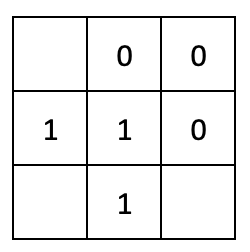
\includegraphics[width=0.8\textwidth]{hit-and-miss-kernel.png}
        \caption{Example of kernel. Cells in blank are "I don't care" valued.}
      \end{figure}
    \end{column}
  \end{columns}
\end{frame}

\begin{frame}[c]
  \frametitle{Morphological Thinning}
  \begin{block}
    {Thinnig operation}
    Given a binary image $I$ and a kernel $K$:
    \begin{equation}
      thin(I, K) = I - hit\mbox{-}or\mbox{-}miss(I, K)
    \end{equation}
    where the subtraction is the logical subtraction $X-Y = X \cap \neg Y$
  \end{block}
  \begin{itemize}
    \item A pixel $(i, j)$ is deleted (i.e. set to 0) if kernel and sub-image \textbf{do not} exacly match, otherwise is left unchanged.
    \item To obtain a skeleton of the image, $thin(I, K)$ should be repeated until no change occurs.
    \item The choice of the kernel determines which pixels are deleted from the region.
  \end{itemize}
\end{frame}

\begin{frame}
  \frametitle{Skeletonization Kernels}
  \begin{itemize}
    \item Recalling Slide~\ref{sli:skeleton} a skeleton should preserve geometric and topological characteristics of the region such as connectivity, holes, cavities etc.
    \item $thin(I, K)$ deletes pixels based on the kernel K.
    \item The two kernels below (and all their 90° rotations) allow to delete only pixels whose deletion preserves the above mentioned characteristics.
    \item In each iteration $thin(I, K)$ is executed for each of the 8 resulting kernels.
  \end{itemize}
  \begin{figure}
    \centering
    \begin{subfigure}[b]{0.45\textwidth}
      \centering
      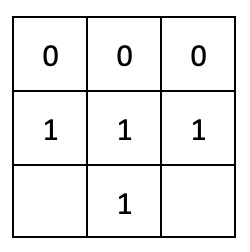
\includegraphics[width=0.6\textwidth]{border-kernel.png}
      \caption{Detects deletable border pixels.}
    \end{subfigure}
    \hfill
    \begin{subfigure}[b]{0.45\textwidth}
      \centering
      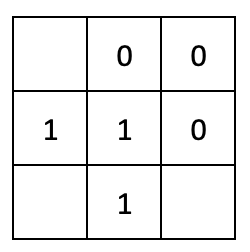
\includegraphics[width=0.6\textwidth]{corner-kernel.png}
      \caption{Detects deletable corner pixels.}
    \end{subfigure}
    \caption{Morphological thinning kernels (and all their 90° rotations)}
  \end{figure}
\end{frame}

\begin{frame}
  \frametitle{Spurs Problem}
  \begin{block}{Spurs}
    Skeletons obtained by $thin(I, K)$ with kernels presented in the previous slide can present \textbf{short spurs} produced by irregularities in the boundary of the region as shown below.
  \end{block}
  \begin{columns}
    \begin{column}{0.4\textwidth}
      \begin{figure}
        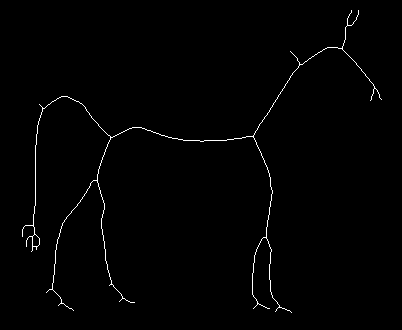
\includegraphics[width=\textwidth]{spur-example.png}
        \caption{Morphological thinning skeleton with spurs.}
      \end{figure}
    \end{column}
    \begin{column}{0.6\textwidth}
      \begin{itemize}
        \item Spurs can be removed by a process called \textbf{pruning}.
        \item Pruning is performed by applying $thin(I, K)$ with ad-hoc kernels for a \textbf{fixed amount} of iterations.
        \item Pruning until convergence would actually remove all pixels exept those which form closed loops.
      \end{itemize}
    \end{column}
  \end{columns}
\end{frame}

\begin{frame}
  \frametitle{Kernels for Spur Removal}
  By using the kernels (and all their 90° rotations) shown below is possible to remove spurs from skeleton.
  \begin{columns}
    \begin{column}{0.5\textwidth}
      \begin{figure}
        \centering
        \begin{subfigure}[b]{0.5\textwidth}
          \centering
          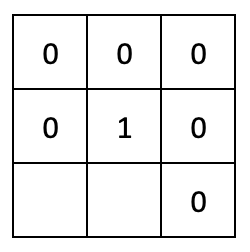
\includegraphics[width=\textwidth]{spur-1-kernel.png}
        \end{subfigure}
        \hfill
        \begin{subfigure}[b]{0.5\textwidth}
          \centering
          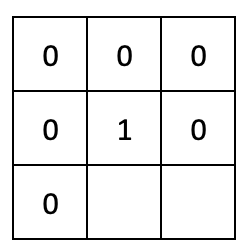
\includegraphics[width=\textwidth]{spur-2-kernel.png}
        \end{subfigure}
        \caption{Spur removal kernels}
      \end{figure}
    \end{column}
    \begin{column}{0.5\textwidth}
      After removing spurs for 10 iterations we get the following skeleton.
      \begin{figure}
        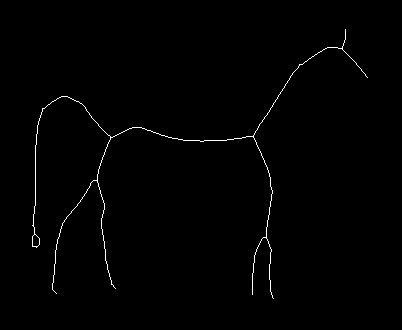
\includegraphics[width=\textwidth]{spur-removed.png}
        \caption{Skeleton after spur removal.}
      \end{figure}
    \end{column}
  \end{columns}
\end{frame}

\begin{frame}
  \frametitle{Morphological Thinning Pseudocode}
  \section{Morphological Thinning}
\begin{frame}
  \frametitle{Morphological Thinning}
  \textbf{Morphological Thinning}~\cite{morph} is a morphological operation that removes contour pixels from a region of a binary image. It relies on the \textbf{Hit-or-Miss transform} operation.
  \begin{block}
    {Hit-or-Miss transform}
    General binary morphological operation used to look for the presence of specific patterns of \emph{foreground} and \emph{background pixels} (1s or 0s respectively).
  \end{block}
  \begin{columns}
    \begin{column}{0.7\textwidth}
      \begin{itemize}
        \item Hit-or-Miss transform uses a \emph{structuring element} or \emph{kernel} to look for those patterns. \item Tipycally it is used a $3\times3$ kernel. It can contain both 1s and 0s and a special "I don't care" value.
        \item Iteration over all pixels, comparing the kernel with the underlying sub-image.
        \item \lstinline{M[i][j]}$= \begin{cases} 1 & \mbox{if } kernel =$ \lstinline{M[i-1:i+1][j-1:j+1]}$ \\ 0 & otherwise\end{cases}$
      \end{itemize}
    \end{column}
    \begin{column}{0.3\textwidth}
      \begin{figure}
        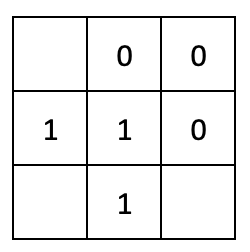
\includegraphics[width=0.8\textwidth]{hit-and-miss-kernel.png}
        \caption{Example of kernel. Cells in blank are "I don't care" valued.}
      \end{figure}
    \end{column}
  \end{columns}
\end{frame}

\begin{frame}[c]
  \frametitle{Morphological Thinning}
  \begin{block}
    {Thinnig operation}
    Given a binary image $I$ and a kernel $K$:
    \begin{equation}
      thin(I, K) = I - hit\mbox{-}or\mbox{-}miss(I, K)
    \end{equation}
    where the subtraction is the logical subtraction $X-Y = X \cap \neg Y$
  \end{block}
  \begin{itemize}
    \item A pixel $(i, j)$ is deleted (i.e. set to 0) if kernel and sub-image \textbf{do not} exacly match, otherwise is left unchanged.
    \item To obtain a skeleton of the image, $thin(I, K)$ should be repeated until no change occurs.
    \item The choice of the kernel determines which pixels are deleted from the region.
  \end{itemize}
\end{frame}

\begin{frame}
  \frametitle{Skeletonization Kernels}
  \begin{itemize}
    \item Recalling Slide~\ref{sli:skeleton} a skeleton should preserve geometric and topological characteristics of the region such as connectivity, holes, cavities etc.
    \item $thin(I, K)$ deletes pixels based on the kernel K.
    \item The two kernels below (and all their 90° rotations) allow to delete only pixels whose deletion preserves the above mentioned characteristics.
    \item In each iteration $thin(I, K)$ is executed for each of the 8 resulting kernels.
  \end{itemize}
  \begin{figure}
    \centering
    \begin{subfigure}[b]{0.45\textwidth}
      \centering
      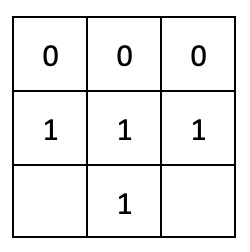
\includegraphics[width=0.6\textwidth]{border-kernel.png}
      \caption{Detects deletable border pixels.}
    \end{subfigure}
    \hfill
    \begin{subfigure}[b]{0.45\textwidth}
      \centering
      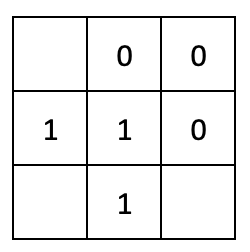
\includegraphics[width=0.6\textwidth]{corner-kernel.png}
      \caption{Detects deletable corner pixels.}
    \end{subfigure}
    \caption{Morphological thinning kernels (and all their 90° rotations)}
  \end{figure}
\end{frame}

\begin{frame}
  \frametitle{Spurs Problem}
  \begin{block}{Spurs}
    Skeletons obtained by $thin(I, K)$ with kernels presented in the previous slide can present \textbf{short spurs} produced by irregularities in the boundary of the region as shown below.
  \end{block}
  \begin{columns}
    \begin{column}{0.4\textwidth}
      \begin{figure}
        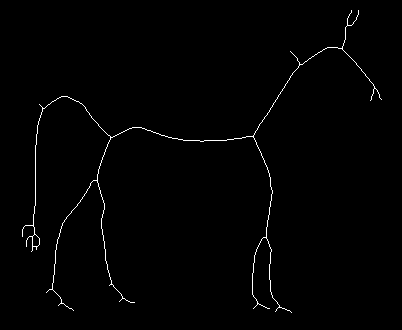
\includegraphics[width=\textwidth]{spur-example.png}
        \caption{Morphological thinning skeleton with spurs.}
      \end{figure}
    \end{column}
    \begin{column}{0.6\textwidth}
      \begin{itemize}
        \item Spurs can be removed by a process called \textbf{pruning}.
        \item Pruning is performed by applying $thin(I, K)$ with ad-hoc kernels for a \textbf{fixed amount} of iterations.
        \item Pruning until convergence would actually remove all pixels exept those which form closed loops.
      \end{itemize}
    \end{column}
  \end{columns}
\end{frame}

\begin{frame}
  \frametitle{Kernels for Spur Removal}
  By using the kernels (and all their 90° rotations) shown below is possible to remove spurs from skeleton.
  \begin{columns}
    \begin{column}{0.5\textwidth}
      \begin{figure}
        \centering
        \begin{subfigure}[b]{0.5\textwidth}
          \centering
          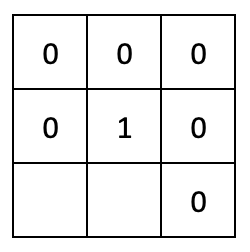
\includegraphics[width=\textwidth]{spur-1-kernel.png}
        \end{subfigure}
        \hfill
        \begin{subfigure}[b]{0.5\textwidth}
          \centering
          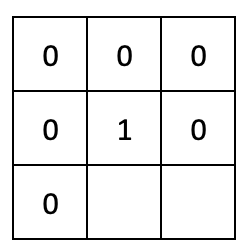
\includegraphics[width=\textwidth]{spur-2-kernel.png}
        \end{subfigure}
        \caption{Spur removal kernels}
      \end{figure}
    \end{column}
    \begin{column}{0.5\textwidth}
      After removing spurs for 10 iterations we get the following skeleton.
      \begin{figure}
        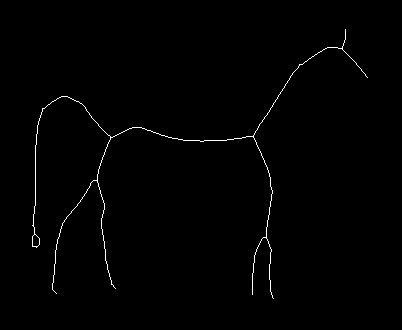
\includegraphics[width=\textwidth]{spur-removed.png}
        \caption{Skeleton after spur removal.}
      \end{figure}
    \end{column}
  \end{columns}
\end{frame}

\begin{frame}
  \frametitle{Morphological Thinning Pseudocode}
  \section{Morphological Thinning}
\begin{frame}
  \frametitle{Morphological Thinning}
  \textbf{Morphological Thinning}~\cite{morph} is a morphological operation that removes contour pixels from a region of a binary image. It relies on the \textbf{Hit-or-Miss transform} operation.
  \begin{block}
    {Hit-or-Miss transform}
    General binary morphological operation used to look for the presence of specific patterns of \emph{foreground} and \emph{background pixels} (1s or 0s respectively).
  \end{block}
  \begin{columns}
    \begin{column}{0.7\textwidth}
      \begin{itemize}
        \item Hit-or-Miss transform uses a \emph{structuring element} or \emph{kernel} to look for those patterns. \item Tipycally it is used a $3\times3$ kernel. It can contain both 1s and 0s and a special "I don't care" value.
        \item Iteration over all pixels, comparing the kernel with the underlying sub-image.
        \item \lstinline{M[i][j]}$= \begin{cases} 1 & \mbox{if } kernel =$ \lstinline{M[i-1:i+1][j-1:j+1]}$ \\ 0 & otherwise\end{cases}$
      \end{itemize}
    \end{column}
    \begin{column}{0.3\textwidth}
      \begin{figure}
        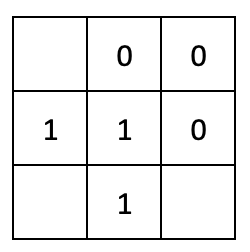
\includegraphics[width=0.8\textwidth]{hit-and-miss-kernel.png}
        \caption{Example of kernel. Cells in blank are "I don't care" valued.}
      \end{figure}
    \end{column}
  \end{columns}
\end{frame}

\begin{frame}[c]
  \frametitle{Morphological Thinning}
  \begin{block}
    {Thinnig operation}
    Given a binary image $I$ and a kernel $K$:
    \begin{equation}
      thin(I, K) = I - hit\mbox{-}or\mbox{-}miss(I, K)
    \end{equation}
    where the subtraction is the logical subtraction $X-Y = X \cap \neg Y$
  \end{block}
  \begin{itemize}
    \item A pixel $(i, j)$ is deleted (i.e. set to 0) if kernel and sub-image \textbf{do not} exacly match, otherwise is left unchanged.
    \item To obtain a skeleton of the image, $thin(I, K)$ should be repeated until no change occurs.
    \item The choice of the kernel determines which pixels are deleted from the region.
  \end{itemize}
\end{frame}

\begin{frame}
  \frametitle{Skeletonization Kernels}
  \begin{itemize}
    \item Recalling Slide~\ref{sli:skeleton} a skeleton should preserve geometric and topological characteristics of the region such as connectivity, holes, cavities etc.
    \item $thin(I, K)$ deletes pixels based on the kernel K.
    \item The two kernels below (and all their 90° rotations) allow to delete only pixels whose deletion preserves the above mentioned characteristics.
    \item In each iteration $thin(I, K)$ is executed for each of the 8 resulting kernels.
  \end{itemize}
  \begin{figure}
    \centering
    \begin{subfigure}[b]{0.45\textwidth}
      \centering
      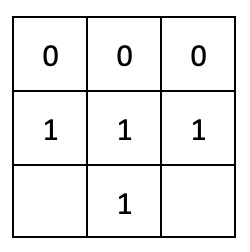
\includegraphics[width=0.6\textwidth]{border-kernel.png}
      \caption{Detects deletable border pixels.}
    \end{subfigure}
    \hfill
    \begin{subfigure}[b]{0.45\textwidth}
      \centering
      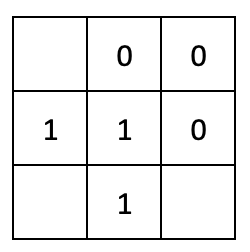
\includegraphics[width=0.6\textwidth]{corner-kernel.png}
      \caption{Detects deletable corner pixels.}
    \end{subfigure}
    \caption{Morphological thinning kernels (and all their 90° rotations)}
  \end{figure}
\end{frame}

\begin{frame}
  \frametitle{Spurs Problem}
  \begin{block}{Spurs}
    Skeletons obtained by $thin(I, K)$ with kernels presented in the previous slide can present \textbf{short spurs} produced by irregularities in the boundary of the region as shown below.
  \end{block}
  \begin{columns}
    \begin{column}{0.4\textwidth}
      \begin{figure}
        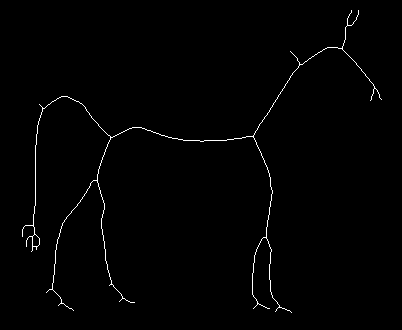
\includegraphics[width=\textwidth]{spur-example.png}
        \caption{Morphological thinning skeleton with spurs.}
      \end{figure}
    \end{column}
    \begin{column}{0.6\textwidth}
      \begin{itemize}
        \item Spurs can be removed by a process called \textbf{pruning}.
        \item Pruning is performed by applying $thin(I, K)$ with ad-hoc kernels for a \textbf{fixed amount} of iterations.
        \item Pruning until convergence would actually remove all pixels exept those which form closed loops.
      \end{itemize}
    \end{column}
  \end{columns}
\end{frame}

\begin{frame}
  \frametitle{Kernels for Spur Removal}
  By using the kernels (and all their 90° rotations) shown below is possible to remove spurs from skeleton.
  \begin{columns}
    \begin{column}{0.5\textwidth}
      \begin{figure}
        \centering
        \begin{subfigure}[b]{0.5\textwidth}
          \centering
          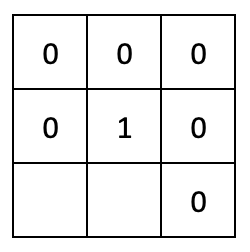
\includegraphics[width=\textwidth]{spur-1-kernel.png}
        \end{subfigure}
        \hfill
        \begin{subfigure}[b]{0.5\textwidth}
          \centering
          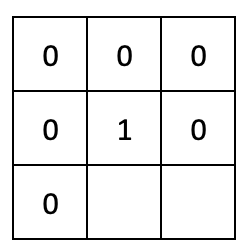
\includegraphics[width=\textwidth]{spur-2-kernel.png}
        \end{subfigure}
        \caption{Spur removal kernels}
      \end{figure}
    \end{column}
    \begin{column}{0.5\textwidth}
      After removing spurs for 10 iterations we get the following skeleton.
      \begin{figure}
        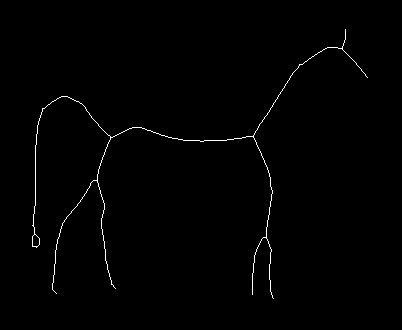
\includegraphics[width=\textwidth]{spur-removed.png}
        \caption{Skeleton after spur removal.}
      \end{figure}
    \end{column}
  \end{columns}
\end{frame}

\begin{frame}
  \frametitle{Morphological Thinning Pseudocode}
  \input{assets/pseudocode/morph.tex}
\end{frame}

\end{frame}

\end{frame}

\end{frame}
